\documentclass{article}

\usepackage{graphicx}
\usepackage{tikz}
\usepackage{tikzsymbols}
\usetikzlibrary{calc,patterns,shapes.geometric}
\pagestyle{empty}
\usepackage[margin=0pt]{geometry}
\geometry{papersize={14in,12in}}

\def\centerarc[#1](#2)(#3:#4:#5){\draw[#1] ($(#2)+({#5*cos(#3)},{#5*sin(#3)})$) arc (#3:#4:#5);}

\begin{document}
	\begin{figure}
		\centering
		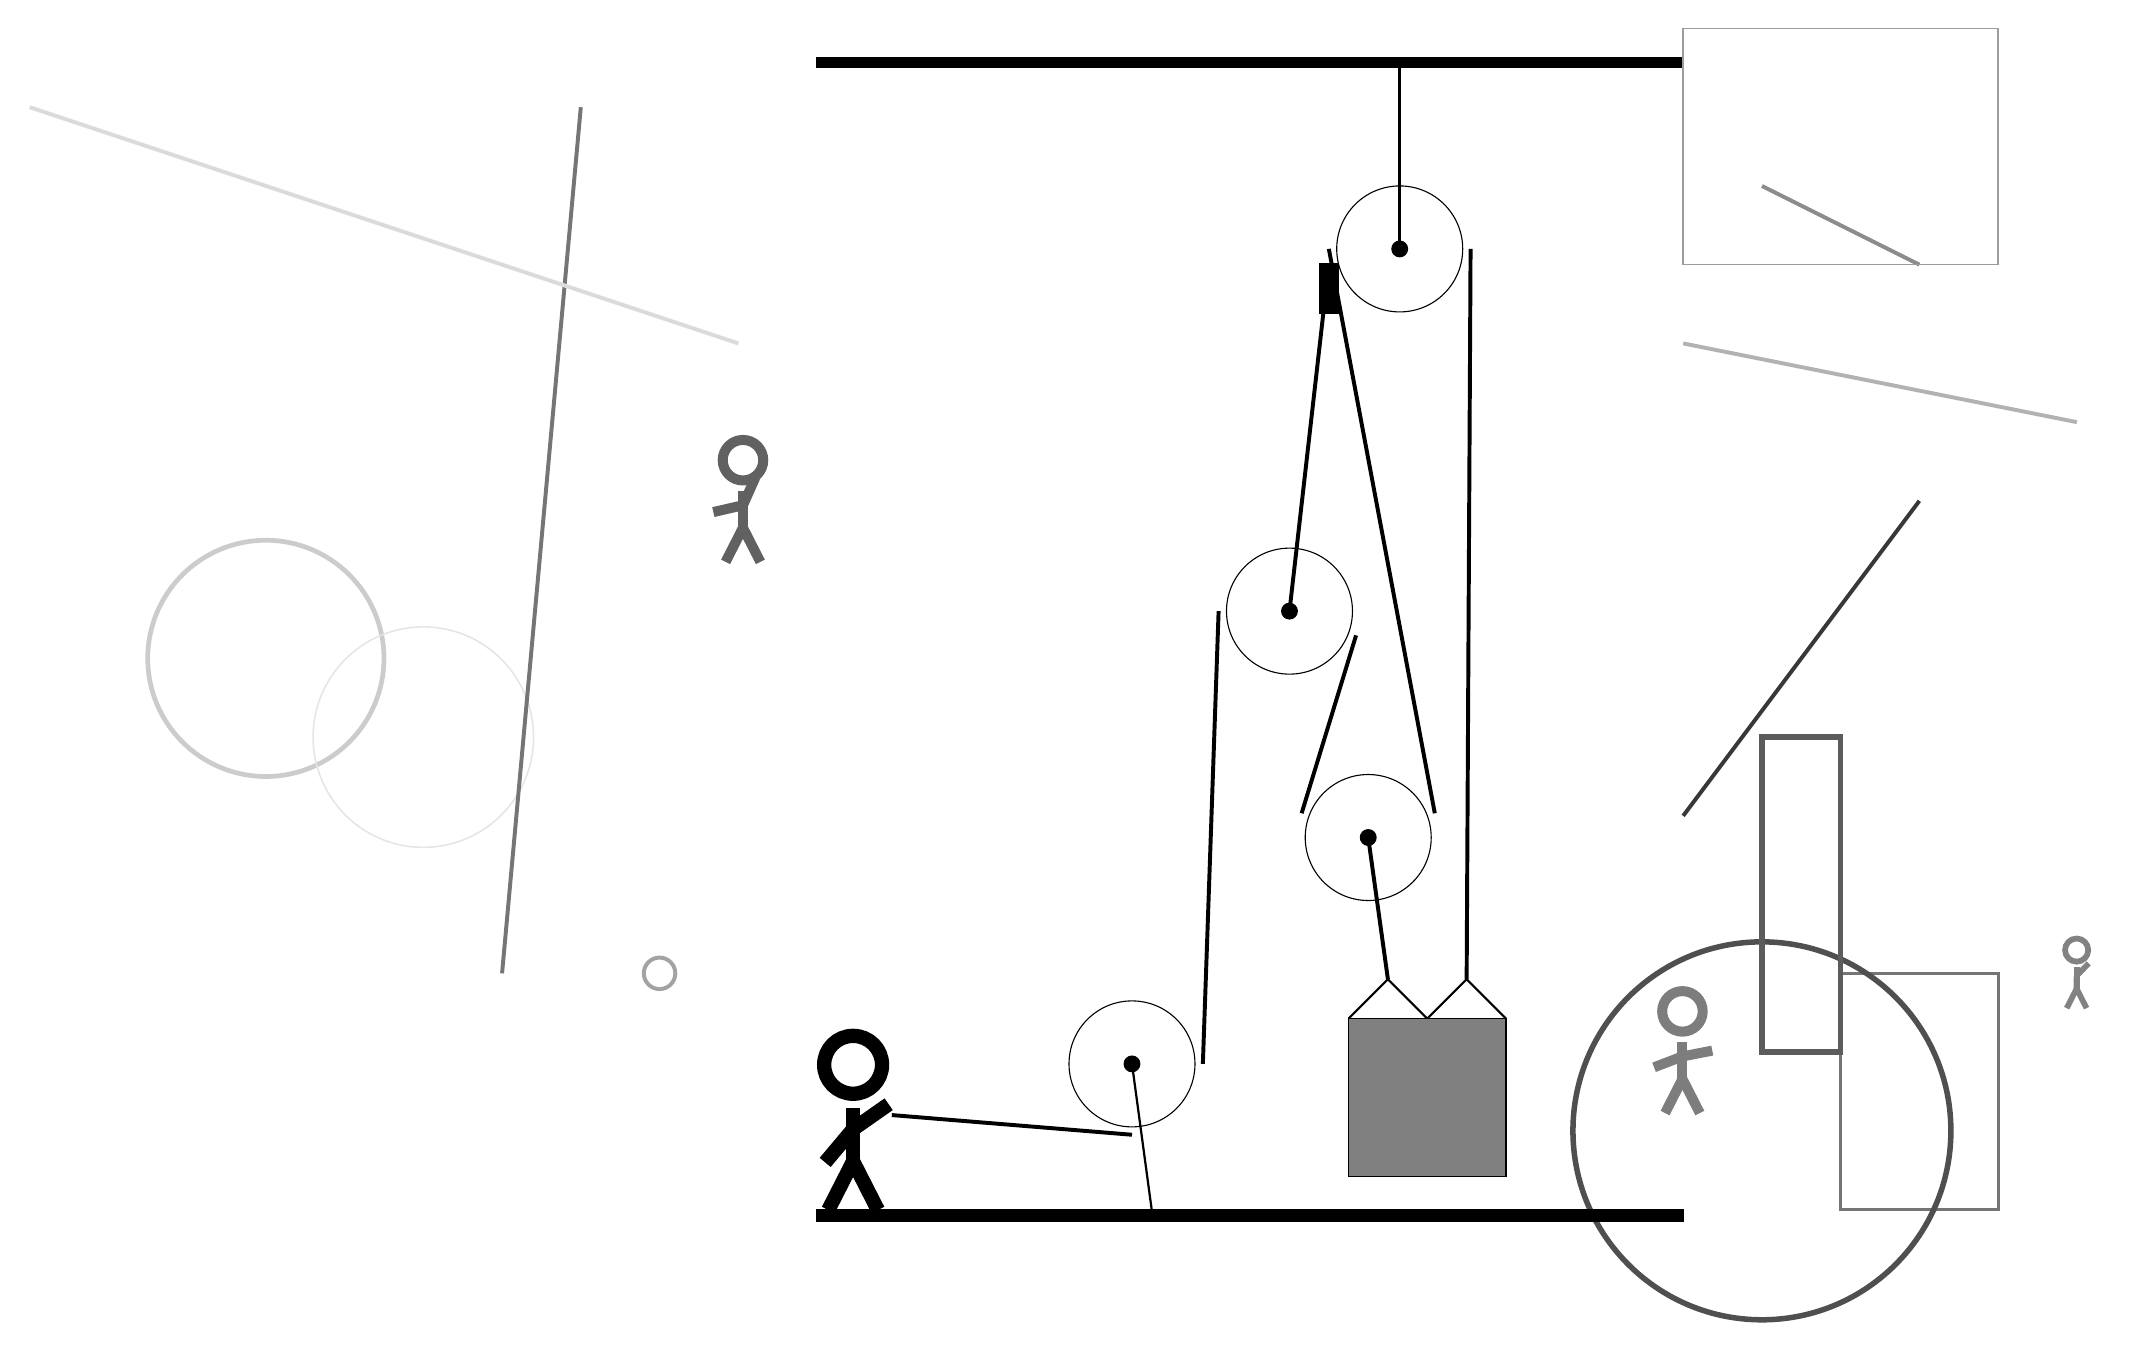
\begin{tikzpicture}
			%%%%% START %%%%%
			
			\draw[fill=black] (-6, 11.5) rectangle (5, 11.625);
			
			\draw (0, 4.6) circle (0.8);
			\draw[fill=black] (0, 4.6) circle (0.1);
			
			\draw (1, 1.725) circle (0.8);
			\draw[fill=black] (1, 1.725) circle (0.1);
			
			\draw (1.4, 9.2) circle (0.8);
			\draw[fill=black] (1.4, 9.2) circle (0.1);
			\draw[very thick] (1.4, 9.2) -- (1.4, 11.5);
			
			\draw (-2, -1.15) circle (0.8);
			\draw[fill=black] (-2, -1.15) circle (0.1);
			\draw[thick] (-2, -1.15) -- (-1.75, -3);
			
			
			\draw[thick]  (0.75, -0.575) -- (1.25, -0.075) -- (1.75, -0.575) -- (2.25, -0.075) -- (2.75, -0.575);
			\draw[fill=black!50] (0.75, -0.575) rectangle (2.75, -2.575);
			\draw[line width=0.5mm] (-5.05, -1.8) -- (-2, -2.05);
			\centerarc[line width=0.5mm](-2, -1.15)(270:360:0.9);
			\draw[line width=0.5mm] (-1.1, -1.15) -- (-0.9, 4.6);
			\draw[line width=0.5mm] (0, 4.6) -- (0.5, 9.0);
			\draw[line width=0.5mm, fill=black](0.4, 8.4) rectangle (0.6, 9.0);
			\centerarc[line width=0.5mm](0, 4.6)(-20:180:0.9);
			\draw[line width=0.5mm] (0.8457, 4.2922) -- (0.1543, 2.0328);
			\centerarc[line width=0.5mm](1, 1.725)(160:380:0.9);
			\draw[line width=0.5mm] (1.8457, 2.0328) -- (0.5, 9.2);
			\draw[line width=0.5mm](1, 1.725) -- (1.25, -0.075);
			\centerarc[line width=0.5mm](1.4, 9.2)(0:180:0.9);
			\draw[line width=0.5mm] (2.3, 9.2) -- (2.25, -0.075);
			
			\node at (-5.5, -1.9) {\Strichmaxerl[10][50][35]};
			
			\draw[line width=0.5mm, color=black!45](8, 9) -- (6, 10);
			
			\draw [line width=0.6mm, color=black!20](-13, 4) circle (1.5);
			\draw [line width=0.2mm, color=black!10](-11, 3) circle (1.4);
			\draw[line width=0.5mm, color=black!78](8, 6) -- (5, 2);
			
			\node[line width=0.5mm, color=black!49] at (10, 0) {\Strichmaxerl[4][89][46]};
			
			\draw[line width=0.5mm, color=black!30](10, 7) -- (5, 8);
			
			\draw[line width=0.4mm, color=black!54] (7, -3) rectangle (9, 0);
			\draw [line width=0.5mm, color=black!36](-8, 0) circle (0.2);
			\node[line width=0.6mm, color=black!51] at (5, -1) {\Strichmaxerl[7][21][11]};
			\draw [line width=0.7mm, color=black!69](6, -2) circle (2.4);
			
			\node[line width=0.5mm, color=black!62] at (-7, 6) {\Strichmaxerl[7][13][66]};
			\draw[line width=0.7mm, color=black!64] (7, 3) rectangle (6, -1);
			\draw[line width=0.2mm, color=black!39] (5, 9) rectangle (9, 12);
			
			\draw[line width=0.5mm, color=black!54](-9, 11) -- (-10, 0);
			\draw[line width=0.5mm, color=black!14](-7, 8) -- (-16, 11);
			
			\draw[fill=black] (-6, -3) rectangle (5, -3.15);
			
			%%%%% END %%%%%
		\end{tikzpicture}
	\end{figure}	
\end{document}